\documentclass[11pt]{exam}
\usepackage[utf8]{inputenc}
\usepackage[a4paper,top=2cm,left=2cm,right=2cm,bottom=2cm]{geometry}
\usepackage{import}
\usepackage[T1]{fontenc}
\usepackage[german,ngerman]{babel}
\usepackage[table]{xcolor}
\usepackage{amsthm, esvect}
\usepackage{mathtools}
\RequirePackage{amssymb, amsfonts, amsmath, latexsym, verbatim, xspace}
\usepackage{systeme}
\usepackage{multicol}
\usepackage{multirow}
\usepackage{framed}
\usepackage{array}
\usepackage{ragged2e}
\usepackage{graphicx}
\usepackage{pdflscape}
\usepackage{epstopdf}
\usepackage{booktabs}
\usepackage{pdfpages}
\usepackage{float} % Allows putting an [H] in \begin{figure} to specify the exact location of the figure
\usepackage{wrapfig} % Allows in-line images such as the example fish picture
\usepackage{tikz, graphicx} % tikz
\usepackage[position=top]{subfig}
\usepackage[bookmarks=true]{hyperref}%Links
\usepackage{enumerate}
\usepackage{enumitem}
\usepackage[german,ruled,vlined,linesnumbered,algosection]{algorithm2e}
\usepackage[labelfont=sf]{caption}
\usepackage{lmodern}
\usepackage{lscape}
\usepackage{tabularx}
\usepackage{systeme}
\usepackage{hhline}
\usepackage{subfiles}
\usepackage{stackengine}
\usepackage{setspace}
\usepackage{MnSymbol}
\usepackage{tcolorbox}
\usepackage{bbm}
\usepackage{url}
\usepackage{xparse}
\usepackage{sectsty}
\usepackage{array}
\usepackage{ragged2e}
\usepackage{listings} %Stellt Code-Snippets sauber dar

% definiert die Sprache
\selectlanguage{German}

% add command for different dates in Swiss fashion
\newcommand{\monthwordlong}[1]{\ifcase#1 \or Januar\or Februar\or März\or April\or Mai\or Juni\or Juli\or August\or September\or Oktober\or November\or Dezember\fi}
\newcommand{\monthwordshort}[1]{\ifcase#1\or Jan\or Feb\or Mar\or Apr\or Mai\or Jun\or Jul\or Aug\or Sept\or Okt\or Nov\or Dez\fi}
\newcommand{\datelong}{\number\day.\:\monthwordlong{\the\month}\:\number\year}
\newcommand{\dateshort}{\number\day.\:\monthwordshort{\the\month}\:\number\year}

% define color of links inside a text
\definecolor{linkblue}{RGB}{0, 0, 80}
\definecolor{plotblue}{RGB}{100, 100, 255}
\definecolor{myblue}{RGB}{8,164,214}
\definecolor{myred}{RGB}{143,42,41}
\definecolor{forestgreen}{RGB}{34,139,34}
\definecolor{highdive}{RGB}{10,169,194}
\definecolor{charcoal}{RGB}{74,74,74}
\hypersetup{
	colorlinks=true,
	linkcolor=linkblue,
	filecolor=magenta,
	urlcolor=plotblue,
	citecolor=linkblue,
	pdfpagemode=FullScreen,
}


\lstdefinestyle{mystyle}{ % definiert den style des Code-Snippets
	%backgroundcolor=\color{backcolour},
	%commentstyle=\color{codegreen},
	%keywordstyle=\color{magenta},
	%numberstyle=\tiny\color{codegray},
	%stringstyle=\color{codepurple},
	basicstyle=\ttfamily\footnotesize,
	breakatwhitespace=false,
	breaklines=true,
	captionpos=b,
	keepspaces=true,
	%numbers=left,
	%numbersep=5pt,
	showspaces=false,
	showstringspaces=false,
	showtabs=false,
	tabsize=4
}
\lstset{style=mystyle}
\qformat{\Large\textbf{Aufgabe \thequestion\hfill\thepoints}}
\newlist{partes}{enumerate}{3}
\setlist[partes]{label=(\alph*)}
\newcommand{\parte}{\item}
\newlist{subpartes}{enumerate}{3}
\setlist[subpartes]{label=\roman*)}
\newcommand{\subparte}{\item}
\setlist[enumerate,1]{%(
	leftmargin=*, itemsep=12pt, label={\textbf{\arabic*.)}}}
\newcommand\answerbox{%%
	\fbox{\rule{2in}{0pt}\rule[-0.1ex]{0pt}{4ex}}}
\pointpoints{Punkt}{Punkte}
\hqword{Frage:}
\hpword{Mögliche Punkte:}
\hsword{Erreicht:}
\htword{Total}
\renewcommand*\half{.5}
\renewcommand{\solutiontitle}{\noindent\textbf{Lösung:}\par\noindent}

% Graphed boxes
\newcommand{\karos}[2]{
  \begin{tikzpicture}
    \draw[step=0.4cm,color=cyan,dotted] (0,0) grid (#1 cm ,#2 cm);
  %  \draw((#1)/2 cm,0)--((#1)/2 cm,/#2)/2cm)
  \end{tikzpicture}
}
\usetikzlibrary{arrows, petri, topaths, graphs}
\linespread{1.2} % Line spacing

%=========================================================
\newenvironment{parcols}[1][]{
    \begin{parts}\begin{multicols}{#1}
}{
    \end{multicols}\end{parts}
}
%=========================================================
\newenvironment{itemcols}[1][]{
	\begin{itemize}\begin{multicols}{#1}
		}{
	\end{multicols}\end{itemize}
}

%=========================================================
\newcommand{\antwort}[1]{
	{\setlength{\textwidth}{\textwidth}\fillwithgrid{#1cm}\vspace{5pt}}
}

%=========================================================
% Karriertes Papier für Antwort MIT OVERLAY
\tcbuselibrary{breakable,skins}
\usetikzlibrary{mindmap,trees}
\newlength\tindent
\setlength{\tindent}{\parindent}
\setlength{\parindent}{0pt}
\setlength{\parskip}{0pt}

\newtcolorbox{gridspace}[1]{%
	enhanced,
	breakable,
	blanker,
	boxrule=0pt,
	left=5mm,
	right=5mm,
	top=5.75mm,
	bottom=0mm,
	boxsep=0pt,
	height=#1cm,
	width=16cm,
	before upper={
		\begingroup
		\setlength{\baselineskip}{5.75mm}
		\setlength{\parskip}{0pt}
		\setlength{\lineskip}{0pt}
		% keep every paragraph on the grid rhythm
		%\everypar{\vspace{0pt}\strut}
		% math formulas shifted by one grid row
		\let\oldbracketopen\[
		\renewcommand{\[}{\vspace{-5mm}\oldbracketopen}
		% Align displayed formulas to the grid
		\setlength{\abovedisplayskip}{0pt}
		\setlength{\belowdisplayskip}{0pt}
		\setlength{\abovedisplayshortskip}{0pt}
		\setlength{\belowdisplayshortskip}{0pt}
		% Enumerate follows the same rhythm
		\setlist[enumerate]{leftmargin=6mm,itemsep=0mm,topsep=0pt,parsep=0pt,partopsep=0pt}
		\setlist[itemize]{leftmargin=6mm,itemsep=10mm,topsep=0pt,parsep=0pt,partopsep=0pt}},
	after upper={
		\endgroup},
	underlay={
		\draw[step=5mm,color=gray!55] (interior.south west) grid (interior.north east);}
}

%%
% Math Arrows
%%
\newcommand{\same}{\ensuremath{\Longleftrightarrow}}
\renewcommand{\to}{\ensuremath{\longrightarrow}}
\newcommand{\qsame}{\quad\same\quad}
\newcommand{\dsame}{\ensuremath{:\Leftrightarrow}}
\newcommand{\qdsame}{\quad\dsame\quad}
\newcommand{\ldsame}{\ensuremath{:\Longleftrightarrow}}
\newcommand{\samedef}{\ensuremath{\us {\text{def}} \Leftrightarrow}}
\newcommand{\qsamedef}{\quad\samedef\quad}
\newcommand{\lsamedef}{\ensuremath{\us {\text{def}} \Longleftrightarrow}}
\newcommand{\qlsamedef}{\quad\lsamedef\quad}


%%
% Mengendefinitionen
%%
\newcommand{\M}{\ensuremath{\mathcal{M}}}
\newcommand{\N}{\ensuremath{\mathbb{N}}}
\newcommand{\Z}{\ensuremath{\mathbb{Z}}}
\newcommand{\Q}{\ensuremath{\mathbb{Q}}}
\newcommand{\I}{\ensuremath{\mathbb{I}}}
\newcommand{\R}{\ensuremath{\mathbb{R}}}
\newcommand{\C}{\ensuremath{\mathbb{C}}}
\renewcommand{\S}{\ensuremath{\mathbb{S}}}
\newcommand{\Prim}{\ensuremath{\mathbb{P}}}
\newcommand{\0}{\ensuremath{\emptyset}}
\renewcommand{\Re}{\ensuremath{\operatorname{Re}}}
\renewcommand{\Im}{\ensuremath{\operatorname{Im}}}
\newcommand{\strich}{\ensuremath{\big\vert}}

%%
% Mengenoperation
%%
\renewcommand{\nin}{\not\in}


%%
% Logisches Und und Oder
%%
\newcommand{\sand}{\ensuremath{\; \land \;}}
\newcommand{\sor}{\ensuremath{\; \lor \;}}
\renewcommand{\*}{\ensuremath{\cdot}}
\newcommand{\oder}{\vee}
\newcommand{\n}{\neg}
\newcommand{\und}{\wedge}


%%
% Bei Integral, Summe,... die Grenzen über bzw.
% unter das Zeichen
%%
\renewcommand{\d}[1]{\ensuremath{\operatorname{d}\!{#1}}}
\newcommand{\Sum}{\sum\limits}
\newcommand{\Prod}{\prod\limits}
\newcommand{\Min}{\min\limits}
\newcommand{\Max}{\max\limits}
\newcommand{\Lim}{\lim\limits}
\newcommand{\Inf}{\inf\limits}
\newcommand{\Sup}{\sup\limits}
\newcommand{\Liminf}{\liminf\limits}
\newcommand{\Limsup}{\limsup\limits}
%\renewcommand{\Cup}{\bigcup\limits}
%\renewcommand{\Cap}{\bigcap\limits}
\newcommand{\Otimes}{\bigotimes\limits}
\newcommand{\Oplus}{\bigoplus\limits}


%%
% Arcus Cotangens, Logarithmus
%%
\let\oldsin\sin
\renewcommand{\sin}[1]{\oldsin{\left(#1\right)}}
\let\oldcos\cos
\renewcommand{\cos}[1]{\oldcos{\left(#1\right)}}
\let\oldtan\tan
\renewcommand{\tan}[1]{\oldtan{\left(#1\right)}}
\let\oldarcsin\arcsin
\renewcommand{\arcsin}[1]{\oldarcsin{\left(#1\right)}}
\let\oldarccos\arccos
\renewcommand{\arccos}[1]{\oldarccos{\left(#1\right)}}
\let\oldarctan\arctan
\renewcommand{\arctan}[1]{\oldarctan{\left(#1\right)}}
\let\oldln\ln
\renewcommand{\ln}[1]{\oldln{\left(#1\right)}}
\newcommand{\Log}[2]{\ensuremath{\operatorname{log}_{#1}\left(#2\right)}}
\newcommand{\e}{\operatorname{e}}
\renewcommand{\exp}[1]{\ensuremath{\operatorname{\e}^{#1}}}


%%
% Griechische Buchstaben
%%
\renewcommand{\epsilon}{\ensuremath{\varepsilon}}
\renewcommand{\phi}{\varphi}
\renewcommand{\l}{\lambda}
\renewcommand{\t}{\tau}


%%
% Bezeichnungen
%%
\newcommand{\Rgn}{\R_{>0}} % R grösser Null
\newcommand{\Rad}{\operatorname{Rad}}   % Radikal
\newcommand{\kgV}{\operatorname{kgV}}   % Kleinster gemeinsame Vielfache
\newcommand{\ggT}{\operatorname{ggT}}   % Grösster gemeinsame Teiler
\newcommand{\winkel}{\sphericalangle}          % Winkelsymbol
\DeclarePairedDelimiter\abs{\lvert}{\rvert} % besserer Betrag
\makeatletter
\let\oldabs\abs
\def\abs{\@ifstar{\oldabs}{\oldabs*}}
\makeatother


%%
% Vektorgeometrie
%%
\renewcommand{\v}[1]{\vv{#1}}       % besserer Pfeil über Buchstaben
\renewcommand{\vec}[2]{\begingroup\renewcommand{\arraystretch}{1}\left(\begin{array}{c} #1 \\ #2 \end{array}\right)\endgroup}   % two dimensional vector
\renewcommand{\Vec}[3]{\begingroup\renewcommand{\arraystretch}{1}\left(\begin{array}{c} #1 \\ #2 \\ #3 \end{array}\right)\endgroup}      % three dimensional vector


%%
% Text
%%
\newcommand*{\Ueq}[1]{\mathrel{\mathop{=}\limits_{\text{#1}}}}
\newcommand*{\Oeq}[1]{\mathrel{\stackrel{\text{#1}}{=}}}
\newcommand{\utext}[2]{\underbrace{#1}_{\substack{#2}}}
\newcommand{\otext}[2]{$\overbrace{\textrm{#1}}^{\textrm{#2}}$}
\newcommand{\lineortext}[1]{\hspace{0,1cm}\underline{\hspace{0.1cm}\hphantom{#1}\hspace{0.1cm}}\hspace{0,1cm}} % Lückentext erstellen
\newcommand{\gap}[1]{\rule{#1 cm}{1pt}}
\pagestyle{headandfoot}
\firstpageheader{}{}{}
\runningheader{\date}{}{\class, \teacher}
\runningheadrule
\firstpagefooter{}{}{}
\runningfooter{}{Viel Erfolg!}{Seite \thepage\:von \numpages}
\runningfootrule
\graphicspath{{images/}}
%=========================================================
\printanswers % falls kommentiert werden die Antwortenfelder angezeigt
\newcommand{\theme}{Integralrechnung}
\newcommand{\teacher}{Jonas Guler}
\newcommand{\class}{4GaMa}
\renewcommand{\date}{16.12.25}
%=========================================================
\begin{document}
\fontsize{14}{14}\selectfont
\begin{questions}
%=========================================================
%-------------------TESTFRAGEN
%=========================================================
\section{Wachstum (ohne TR)}
	\noaddpoints
	\question[\totalpoints]
	\addpoints
	Salmonellen sind Bakterien, die schwere Magen-Darm Erkrankungen auslösen. Bei Temperaturen von über $8^\circ$C vermehren sich Salmonellen exponentiell. Die infektiöse Dosis beträgt ca. eine Million Keime.\newline Bei einem infizierten Ei werden um 10:00 Uhr $1000$ Keime gezählt, um 12:00 Uhr sind es bereits $16000$.
	\begin{parts}
		\part[1] Gib eine Funktion an, mit welcher sich die Anzahl Keime nach $t$ Stunden ausgehend von 10:00 Uhr berechnen lässt.
		\part[1] Bestimme die Zeit, in der sich die Keimzahl verdoppelt?
		\part[3] Um 13:00 Uhr wird das Ei in ein Kühlfach mit $12^\circ$C gelegt. Das bewirkt, dass die Verdopplungszeit\footnote{Die Verdopplungszeit bezeichnet die Zeitspanne, nach der sich der Bestand einer exponentiell wachsende Grösse verdoppelt hat.} doppelt so lange wie bei Raumtemperatur dauert. Berechne, wie lange es geht, bis die infektiöse Dosis an Keimen erreicht ist.
	\end{parts}

	\ifthenelse{\boolean{printanswers}}
	{\begin{solution}
		\begin{parts}
			\part $f(t)=1000\*4^t$
			\part Verdoppelungszeit $\tau=30$ Minuten
			\part $t=\Log{2}{\frac{10^3}{64}}\approx 3.966$ Stunden
		\end{parts}
	\end{solution}}
	{\vspace{5pt}\antwort{2.5}}

%---------------------------------------------------------
\section{Wachstum (mit TR)}
	\noaddpoints
	\question[\totalpoints]
	\addpoints
	Ein durch $10$t chemische Schadstoffe verunreinigter See kann jährlich $10$\% des noch vorhandenen Schadstoffes abbauen.
	\begin{parts}
		\part[1] Stelle eine Formel für die vorhandene Schadstoffmenge $s(x)$ nach $x$ Jahren auf.
		\part[1] Welche Menge Schadstoff wird nach $10$ Jahren im See noch vorhanden sein?
		\part[1] Wenn die Schadstoffmenge im See noch $1$ Prozent des Anfangswertes beträgt,
		dann wird der See wieder zum Baden frei gegeben. Wann wird dies der Fall
		sein?
		\part[1] Bei einer Messung nach $10$ Jahren wird der berechnete Wert von $b)$ um $20$\%
		überschritten. Aufgrund eines Fischsterbens $2$ Jahre zuvor vermutet man, dass
		jemand erneut Chemikalien in den See gegossen hat. Wie viele Tonnen wären
		dies gewesen?
	\end{parts}

	\ifthenelse{\boolean{printanswers}}
	{\begin{solution}
		\begin{parts}
			\part $s(x)=10\*0.9^x$
			\part $s(10)=10\*0.9^{10}\approx 3.487$t
			\part $s(x)=10\*0.9^x=0.1 \quad\Rightarrow\quad x\approx 43.71$y
			\part neuer Wert nach 10 y: $s_n(10)=s(10)\*1.2=4.18$t \newline neuer Wert nach 8 y: $s_n(8)=s_n(10)*0.9^{-2}=5.17$t \newline Vergleich mit Wert nach 8 y: $s_n(8)-s(8)=860.93$kg
		\end{parts}
	\end{solution}}
	{\vspace{5pt}\antwort{2.5}}

%---------------------------------------------------------
	\noaddpoints
	\question[\totalpoints]
	\addpoints
	Wir nehmen an, jemand schluckt eine Tablette Aspirin mit $500$mg Wirkstoff pro Tag. Nach etwa einer Stunde ist die volle Dosis im Blut und entfaltet ihre Wirkung. Die Wirkstoffkonzentration im Blut nimmt pro Stunde um $16\%$ ab. Beträgt die Wirkstoffkonzentration im Blut weniger als die Hälfte des Initialwertes, so wirkt es im Körper nicht mehr schmerzlindernd.
	\begin{parts}
		\part[1] Gib eine Funktionsgleichung an, die den Konzentrationsverlauf ab der maximalen Wirkstoffkonzentration beschreibt, wenn unsere Versuchsperson genau eine solche Tablette pro Tag einnimmt.
		\part[1] Wie viele Stunden wirkt eine einzige Tablette?
		\part[2] Nehmen wir an, bei einer Tablette Aspririn mit doppelter Menge Wirkstoff wird die Halbwertszeit der Wirkstoffkonzentration im Blut vervierfacht. Kann diese Tablette einen gesamten Arbeitstag ($8$ Stunden) schmerzlindernd wirken? Begründe.
	\end{parts}

	\ifthenelse{\boolean{printanswers}}
	{\begin{solution}
			\begin{parts}
				\part $f(t)=c_{max}\*0.84^t$
				\part $\frac{1}{2}\*c_{max}=c_{max}\*0.84^t \quad\Rightarrow\quad t\approx3.98$h
				\part Ja, wird sie, denn $\frac{1}{2}\*C_{max}=C_{max}\*\sqrt[4]{0.84}^t\quad\Rightarrow\quad t\approx35.9$h
			\end{parts}
	\end{solution}}
	{\vspace{5pt}\antwort{2.5}}

%=========================================================
\newpage
\section{Folgen und Reihen (ohne TR)}
	\noaddpoints
	\question[\totalpoints]
	\addpoints
	Gegeben ist die folgende Zahlenpyramide.
	\begin{figure}[H]
		\centering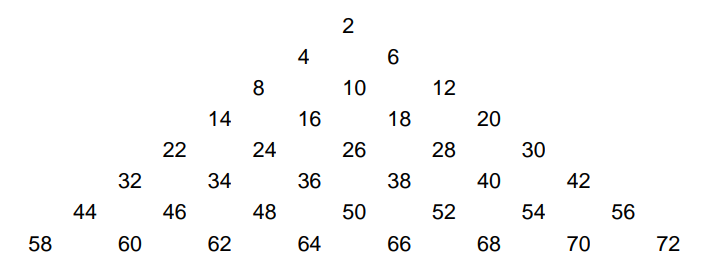
\includegraphics[scale=0.65]{zahlenpyramide.png}
	\end{figure}
	\begin{parts}
		\part[1\half] Berechne die Summe aller notierten Zahlen.
		\part[2\half] Die Zahlen $a_1=2, a_2=4, a_3=8,\ldots$ am linken Rand der Zahlenpyramide können durch $a_n=p\*n^2+q\*n+r$ beschrieben werden.\\ Berechne $p,q,r$.
		\part[2] $b_1,b_2,b_3,\ldots b_{100}$ sind von links nach rechts die Zahlen in der $100.$ Zeile des Dreiecks. Berechne die Summe $b_1+b_2+\ldots+b_{99}$.
	\end{parts}

	\ifthenelse{\boolean{printanswers}}
	{\begin{solution}
		\begin{parts}
			\part Summe$=1332$
			\part $p=1,q=-1,r=2$
			\part $b_1+b_2+\ldots+b_{99}=500'000$
		\end{parts}
	\end{solution}}
	{\vspace{5pt}\antwort{2.5}}

%---------------------------------------------------------
\section{Folgen und Reihen (mit TR)}
	\noaddpoints
	\question[\totalpoints]
	\addpoints
	In der nachfolgenden Figur hat der grösste Halbkreis den Radius $r_1=1$, der zweitgrösste Halbkreis hat den Radius $r_2$.
	\begin{parts}
		\part[1] Zeige, dass $r_s=\frac{1}{\sqrt{2}}$.
		\part[2] Berechne die Summe des Flächeninhalts der farbig hervorgehobenen Flächen ($5$ kleiner
		werdende \flqq Brücken\frqq).
		\part[1] Der Prozess der kleiner werdenden \flqq Brücken\frqq\:kann fortgesetzt werden, sodass unendlich viele \flqq Brücken\frqq\:entstehen. Wie gross ist die Summe des Flächeninhalts der unendlich vielen \flqq Brücken\frqq?
		\part[1] Wie viele \flqq Brücken\frqq\:müssten mindestens gezeichnet werden, bis die kleinste \flqq Brücke\frqq\:weniger als $1$ Promille des Flächeninhaltes der grössten beträgt?
	\end{parts}
	\begin{figure}[H]
		\centering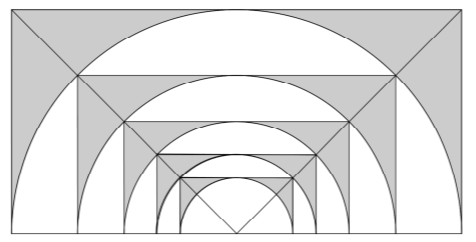
\includegraphics[scale=0.8]{unendliche-brücken.png}
	\end{figure}

	\ifthenelse{\boolean{printanswers}}
	{\begin{solution}
		\begin{parts}
			\part $r_2$ ist die Kathete im gleichschenkligen, rechtwinkligen Dreieck mit Hypothenuse $1$.
			\part Flächeninhalt bildet eine geometrische Folge mit $A_1=2-\frac{\pi}{2}$ und $q=\frac{1}{2}$. Also $s_5=0.8316$.
			\part $s=2\*A_1\approx 0.8584$
			\part $A_n<\frac{1}{1000}\*A_1 \Leftarrow n=11$
		\end{parts}
	\end{solution}}
	{\vspace{5pt}\antwort{2.5}}

%---------------------------------------------------------
	\noaddpoints
	\question[\totalpoints]
	\addpoints
	Das Dreieck $ABC$ und alle unendlich vielen grauen Dreiecke sind gleichschenklig. Wir nehmen an, die Grundlinien und Höhen aller Dreiecke bilden eine unendliche geometrische Folge.
	\begin{parts}
		\part[1] Berechne $\overline{DE}$.
		\part[2] Wie gross ist die Summe der Umfänge aller grauen Dreiecke?
		\part[2] Welchen Bruchteil macht der Flächeninhalt aller grauen Dreiecke von der Dreiecksfläche $ABC$ aus?
	\end{parts}
	\begin{figure}[H]
		\centering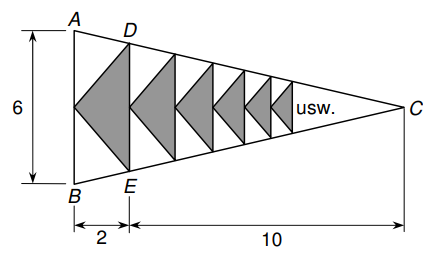
\includegraphics[scale=0.8]{verschachtelte-dreiecke.png}
	\end{figure}

	\ifthenelse{\boolean{printanswers}}
	{\begin{solution}
			\begin{parts}
				\part $\overline{DE}=5$
				\part $U=68.418$
				\part $\frac{A}{A_{\triangle ABC}}=\frac{\frac{5}{1-\frac{25}{36}}}{36}=\frac{5}{11}$
			\end{parts}
	\end{solution}}
	{\vspace{5pt}\antwort{2.5}}

\end{questions}
\end{document}
